\documentclass[notheorems,xetex]{beamer}
%\documentclass[UTF8]{ctexbeamer}
\usepackage{xeCJK}%preamble part
%\usepackage{showframe}
\usepackage{amsmath, amsthm, amssymb}
\usepackage{graphicx}
\usepackage{bm}
\usepackage{caption}
\usepackage{ragged2e}
\usepackage{multirow}
\usepackage{float}
\usepackage{color}
\usepackage{listings}
\lstdefinestyle{lstStyleBase}{%
   basicstyle=\small\ttfamily,
   aboveskip=\medskipamount,
   belowskip=\medskipamount,
   lineskip=0pt,
   boxpos=c,
   showlines=false,
   extendedchars=true,
   upquote=true,
   tabsize=2,
   showtabs=false,
   showspaces=false,
   showstringspaces=false,
   numbers=none,
   linewidth=\linewidth,
   xleftmargin=4pt,
   xrightmargin=0pt,
   resetmargins=false,
   breaklines=true,
   breakatwhitespace=false,
   breakindent=0pt,
   breakautoindent=true,
   columns=flexible,
   keepspaces=true,
   gobble=2,
   framesep=3pt,
   rulesep=1pt,
   framerule=1pt,
   backgroundcolor=\color{gray!5},
   stringstyle=\color{green!40!black!100},
   keywordstyle=\bfseries\color{blue!50!black},
   commentstyle=\slshape\color{black!60}}

\lstdefinestyle{lstStyleShell}{%
   style=lstStyleBase,
   frame=l,
   rulecolor=\color{purple},
   language=bash}
%\usepackage[font=Helv,timeinterval=3]{tdclock}
\DeclareMathOperator*{\rgmax}{argmax}
\DeclareMathOperator*{\rgmin}{argmin}
\DeclareMathOperator{\tr}{tr}
%\setCJKmainfont{SimSun}[AutoFakeBold=false]
%\setsansfont{SimSun}
\setbeamertemplate{frametitle}[default][center]
\setbeamertemplate{footline}[frame number]
\setlength{\parindent}{0.8cm}
%\newcommand{\transpose}[1]{\ensuremath{#1^{\scriptscriptstyle T}}}
\usetheme{Lab2C}
\title{GitHub 高级用法介绍} % (optional, use only with long paper titles)
\author[赵丰]
{\quad {赵丰}\\ \and {zhaofeng-shu33}}
\institute[清华大学] % (optional, but mostly needed)
{\normalsize\quad
  Lab2c 服务器使用培训
}
\date{\the\year 年 \the\month 月 \the\day 日}
%\AtBeginSubsection[]
%{
%  \begin{frame}<beamer>{目录}
%    \tableofcontents[currentsection,currentsubsection]
%  \end{frame}
%}


\begin{document}
\frame{\titlepage}
\frame{\tableofcontents}
%\date{\hspace{1mm} \timemark}
\section{GitHub 中的个人与组织}
\begin{frame}{GitHub 个人主页}
\begin{itemize}
	\item \url{https://github.com/your_github_id}
	\item 活跃程度
     \begin{figure}
	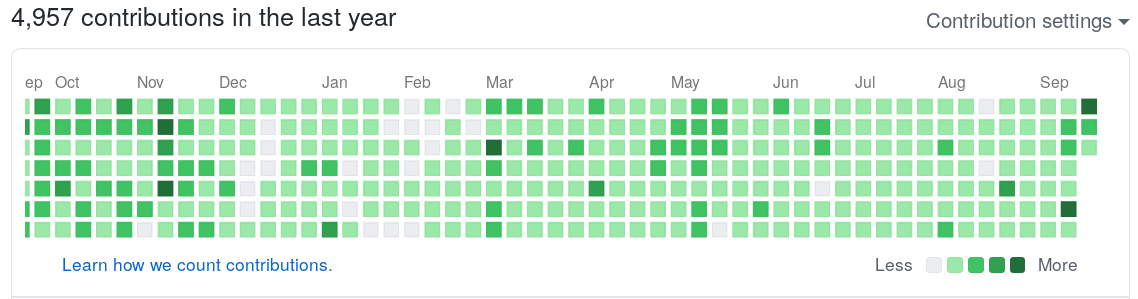
\includegraphics[height=2.5cm]{activity.png}
	\caption*{颜色越深,提交次数越多}
	\end{figure}
	\item 你关注的人与关注你的人
	\begin{figure}
	
\includegraphics[height=1cm]{ff.png}	
	\end{figure}
\end{itemize}
\end{frame}
\begin{frame}{GitHub 组织}
     \begin{figure}
	    \centering
		
\includegraphics[height=2cm]{org.png}
	\end{figure}
\begin{itemize}
	\item 我们的组织 ID: \textbf{mace\_cream}
	\item 置顶的仓库: \textbf{clusterhowto}
	
	\url{https://github.com/mace_cream/clusterhowto}
	\item 接收邀请后,选择自己的可见性: \textbf{公开}或\textbf{仅内部成员可见}。
\end{itemize}
\end{frame}
\section{典型场景}
\frame{\tableofcontents[currentsection]}
\begin{frame}{如何倒退}
\begin{itemize}
	\item 前提: 经常 commit
	\item 倒退命令
	\begin{enumerate}
		\item 暂存当前修改: \texttt{git branch bad\_code}
		\item 回退到想要的地方: \texttt{git reset --hard commit\_hash}
	\end{enumerate}
	\item 撤消倒退 \texttt{git reset --hard bad\_code}
\end{itemize}
\begin{figure}
	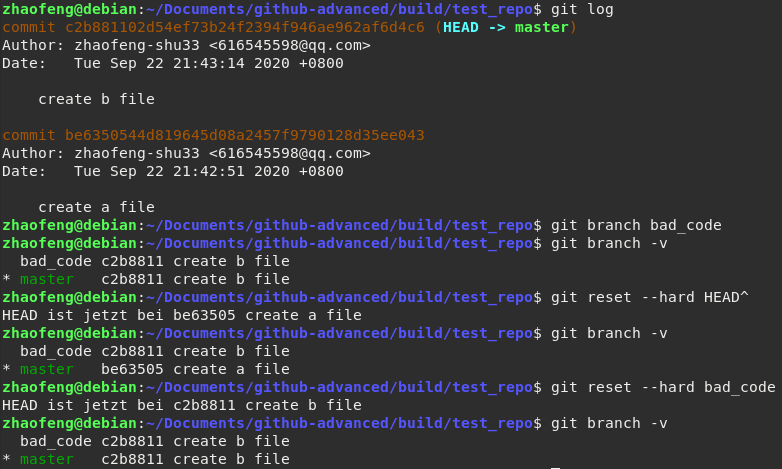
\includegraphics[height=3.5cm]{example_reset.png}
\end{figure}
\end{frame}

\begin{frame}{如何使用 tag}
\begin{itemize}
	\item tags 对应 GitHub 上的 Releases
	\item 使用场景: 软件新版本的发布
	\item 简单 tag 命令: \texttt{git tag v1.0}
	\item 将本地的 tags 推到 GitHub 上: \texttt{git push --tags origin}
\end{itemize}
\begin{figure}
	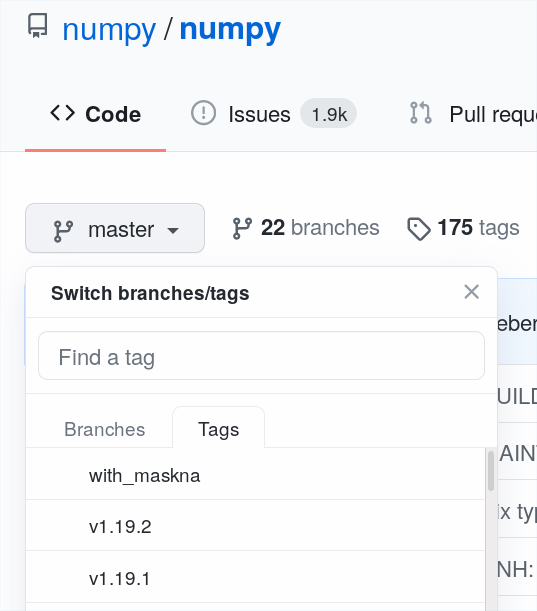
\includegraphics[height=4cm]{numpy_tags.png}
	\caption{numpy 仓库中的 tags}
\end{figure}
\end{frame}
\section{实例分析}
\frame{\tableofcontents[currentsection]}
\begin{frame}[fragile]{merge 中正确解决 conflict}
\begin{itemize}
\item 两个不同的 commit 对同一行代码改动产生了冲突
     \begin{figure}
	\centering
	
\includegraphics[height=0.5cm]{conflict.png}
	\end{figure}
\item 冲突复现
\end{itemize}
\begin{lstlisting}[language=bash]
git clone https://github.com/wuhan2020/\
wuhan2020-frontend-react-app.git
git checkout 801a4e3 -b feature
git checkout 9d11a11 -b main
git merge feature
\end{lstlisting}

\end{frame}
\begin{frame}{冲突现象}

\begin{figure}
	\centering
	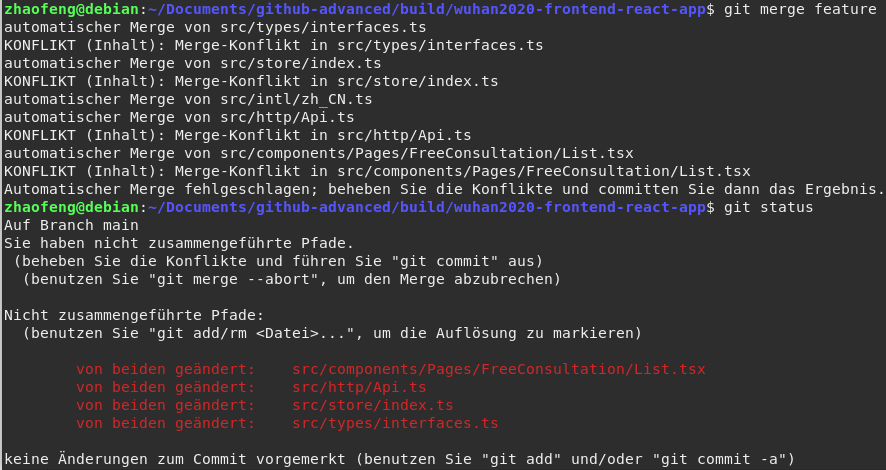
\includegraphics[height=6cm]{phenomenon.png}
\end{figure}
\end{frame}
\begin{frame}{冲突原因}
\begin{figure}
	\centering
	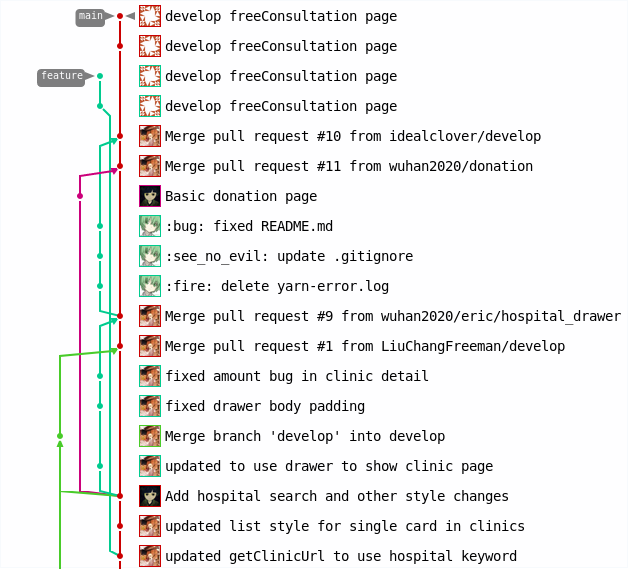
\includegraphics[height=7cm]{deps.png}
\end{figure}
\end{frame}
\begin{frame}{如何解决}
\begin{itemize}
	\item 使用 IDE 工具选择接受哪一部分的改动
\end{itemize}
\begin{figure}
	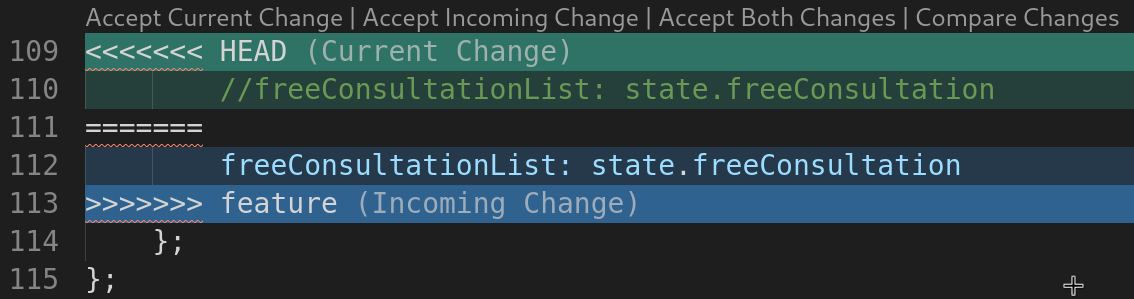
\includegraphics[height=2.5cm]{accept_incoming.png}
\end{figure}

\end{frame}
\begin{frame}{最终效果}
\begin{figure}
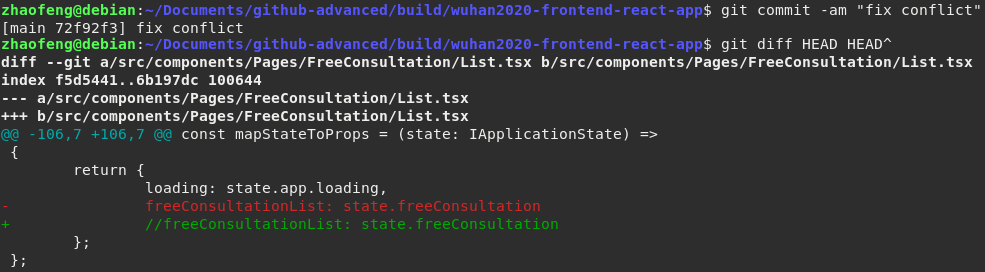
\includegraphics[height=2.5cm]{recover_changes.png}
\caption{复现效果}
\end{figure}
\begin{center}
feature 分支仅贡献一处改动
\end{center}
\begin{figure}
	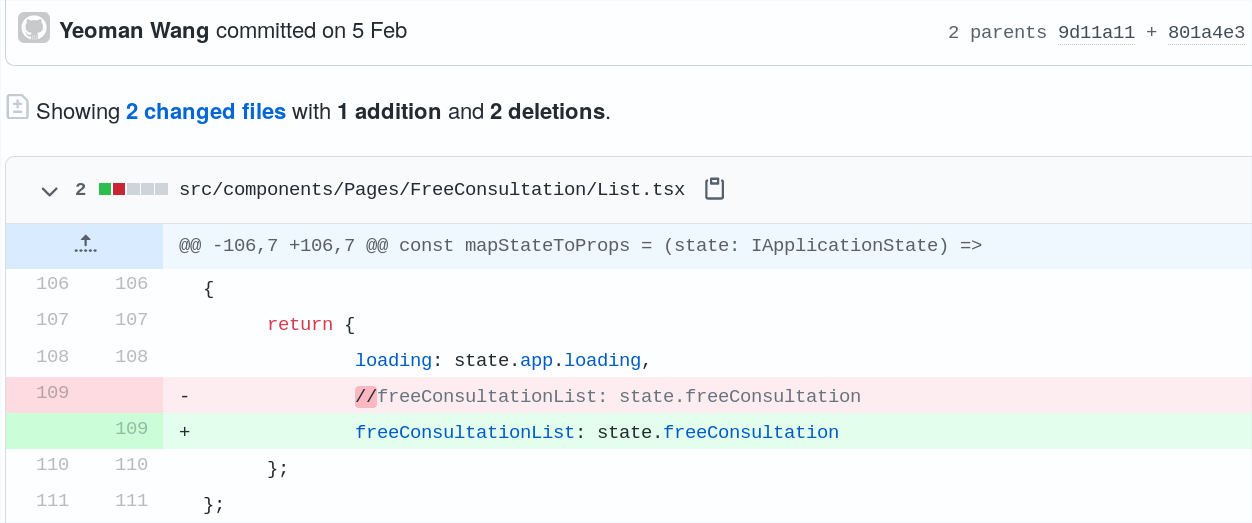
\includegraphics[height=2.5cm]{original.png}
	\caption{原有效果}
\end{figure}
\end{frame}



%\begin{frame}{GitHub Action}

%\end{frame}


\end{document}